\documentclass{article}
\usepackage{tikz}
\usepackage{stanli}
\usepackage{amsmath,amssymb}
\usepackage{graphicx}

\makeatletter

\newcommand*\curveplus{%
  \mathbin{\rotatebox[origin=c]{90}{$\m@th\curvearrowleft$}+}}

\newcommand*\rightplus{%
  \mathpalette\@rightplus\relax}
\newcommand*\@rightplus[1]{%
  \mathbin{\vcenter{\hbox{$\m@th\overset{#1+}{\to}$}}}}

\newcommand*\upplus{%
  \mathbin{+\mathord\uparrow}}

\makeatother

\begin{document}

\title{Spaghetti Bridge Final Report}
\author{Louis Pilgrim(s3776723)\\Nicholas Doublet(s3782672)\\Yassin Elahg(s3783329)\\Jacob Holmes(s3782047)}
\date{31 May, 2019}
\maketitle
\newpage

\section{Executive Summary}

\newpage
\tableofcontents
\newpage

\section{Scope}
\section{Conceptual Design}
\subsection{Spaghetti Testing}
\subsection{Prototype testing}
\subsection{Summary}

\section{Material Selection}
\subsection{Design of Experiments}
\subsection{Results}

\section{Prototype Testing}
\subsection{Fabrication}
\subsection{Testing}
\subsection{Summary}

\section{Force Analysis}
\subsection{External Loading}
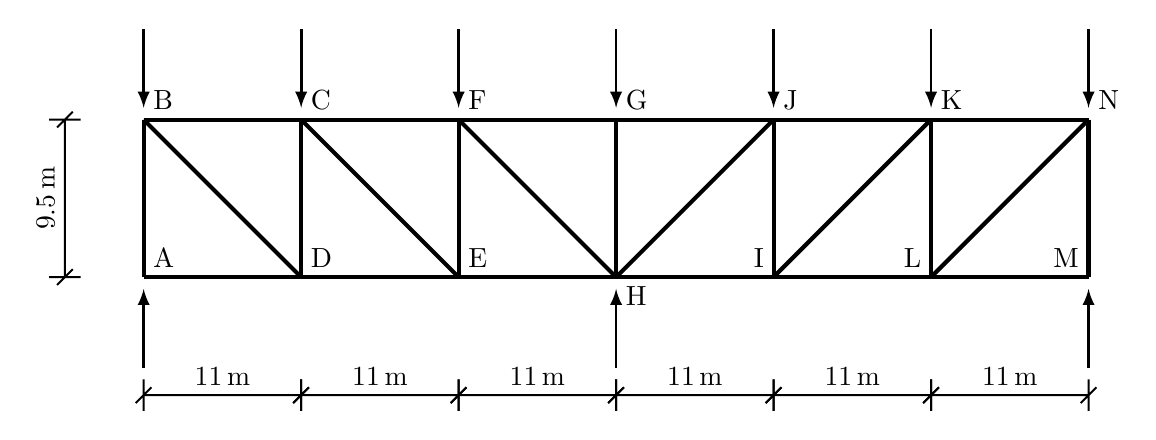
\begin{tikzpicture}
  \scaling{2}
  \point{a}{0}{0};
  \point{b}{0}{1};
  \point{c}{1}{1};
  \point{d}{1}{0};
  \point{e}{2}{0};
  \point{f}{2}{1};
  \point{g}{3}{1};
  \point{h}{3}{0};
  \point{i}{4}{0};
  \point{j}{4}{1};
  \point{k}{5}{1};
  \point{l}{5}{0};
  \point{m}{6}{0};
  \point{n}{6}{1};
  \beam{2}{a}{m};
  \beam{2}{b}{n};
  \beam{2}{a}{b};
  \beam{2}{n}{m};
  \beam{2}{c}{d};
  \beam{2}{f}{e};
  \beam{2}{g}{h};
  \beam{2}{i}{j};
  \beam{2}{l}{k};
  \beam{2}{b}{d};
  \beam{2}{c}{e};
  \beam{2}{f}{h};
  \beam{2}{h}{j};
  \beam{2}{i}{k};
  \beam{2}{l}{n};
  \load{1}{a}[270];
  \load{1}{m}[270];
  \load{1}{h}[270];
  \load{1}{b}[90];
  \load{1}{c}[90];
  \load{1}{f}[90];
  \load{1}{g}[90];
  \load{1}{j}[90];
  \load{1}{k}[90];
  \load{1}{n}[90];
  \dimensioning{1}{a}{d}{-1.5}[$11$\,m]  \dimensioning{1}{d}{e}{-1.5}[$11$\,m]  \dimensioning{1}{e}{h}{-1.5}[$11$\,m]  \dimensioning{1}{h}{i}{-1.5}[$11$\,m]  \dimensioning{1}{i}{l}{-1.5}[$11$\,m]  \dimensioning{1}{l}{m}{-1.5}[$11$\,m]  \dimensioning{2}{a}{b}{-1}[$9.5$\,m]
  \notation{1}{a}{A}
  \notation{1}{b}{B}
  \notation{1}{c}{C}
  \notation{1}{d}{D}
  \notation{1}{e}{E}  \notation{1}{f}{F}
  \notation{1}{g}{G}
  \notation{1}{h}{H}[below right]
  \notation{1}{i}{I}[above left]
  \notation{1}{j}{J}
  \notation{1}{k}{K}
  \notation{1}{l}{L} [above left] \notation{1}{m}{M}[above left]
  \notation{1}{n}{N}
\end{tikzpicture}
The figure above depicts the free body diagram of our bridge design. Where $A_y$ and $M_y$ are the reaction forces, the forces perpendicular to the beam $B-N$ are a spread out load of the weight of the bridge and the road which is $(0.142+0.780)g$. In all the calculations $g=9.81$N\\
First we calculate the individual weight values at each point along the top.
\begin{align*}
    B_y=C_y=F_y=G_y=J_y=K_y=N_y&=\frac{W}{7}\\
    W &=\frac{142+780}{1000}\times g\\
    W &=9.04482\text{N}\\
    B_y=C_y=F_y=G_y=J_y=K_y=N_y&=1.29212\text{N}
\end{align*}
Now we can calculate the reaction forces at $A_y$ and $M_y$.
\begin{align*}
    \curveplus \Sigma M_A=0&=-W_{total} \times 0.33 + M_y \times 0.66\\
    \curveplus \Sigma M_A=0&=-2.984791 + M_y \times 0.66\\
    \curveplus \Sigma M_A=2.984791&=M_y \times 0.66\\
    \curveplus \Sigma M_A=4.52241&=M_y=A_y\\
\end{align*}
\subsection{Internal Loading}
For the calculation of the internal loading we will use the method of joints. We initially started with point:$A$.\\
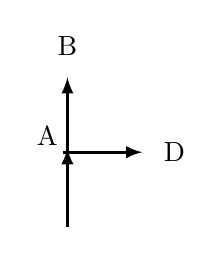
\begin{tikzpicture}
  \scaling{2}
  \point{a}{0}{0};
  \point{b}{0}{.45};
  \point{c}{.55}{-0.1};
  \load{1}{b}[270];
  \load{1}{a}[270];
  \load{1}{c}[180];
  \notation{1}{a}{A}[left]
  \notation{1}{c}{D}[right]
  \notation{1}{b}{B}[above]
\end{tikzpicture}\\
As you can see from this diagram, the summation of forces is very simple and will easily give us the force of both $F_{AB}$ and $F_{AD}$.
\begin{align*}
    \Sigma F_{y}=0&=A_y+F_{AB}\\
    \Sigma F_{y}=F_{AB}&=-A_y\\
    \Sigma F_{y}=F_{AB}&=-4.52241\text{N}\\
    \Sigma F_{y}=F_{AB}&=4.52241\text{N in compression}\\
    \Sigma F_{x}=0&=F_{AD}\\
\end{align*}
We can then use this same process to find out the forces on each member in the diagram which is shown below. It is important to note that this bridge is symmetrical along the $H-G$ beam meaning that we only had the calculate one side in order to also find out the forces on each member on the other side.\\

Internal Force diagram where blue is compression and red is tension.\\
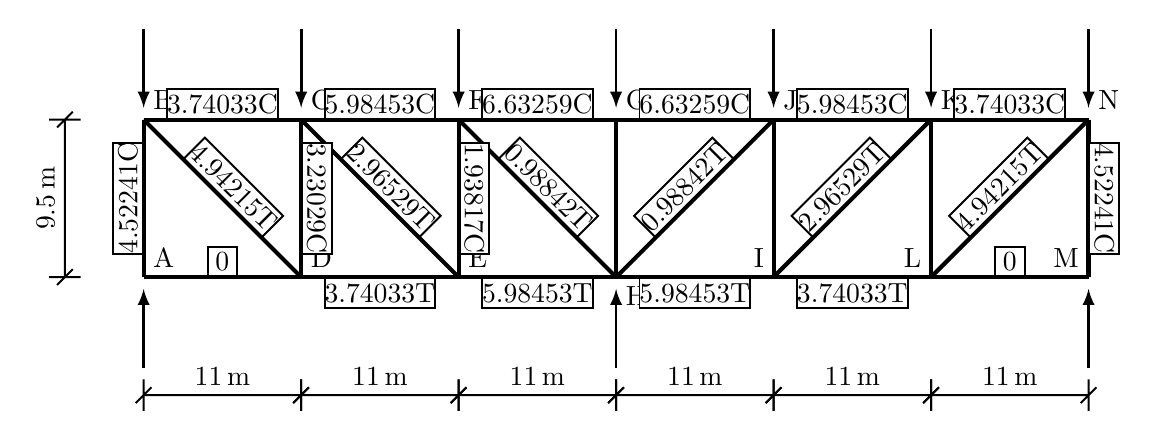
\begin{tikzpicture}
  \scaling{2}
  \point{a}{0}{0};
  \point{b}{0}{1};
  \point{c}{1}{1};
  \point{d}{1}{0};
  \point{e}{2}{0};
  \point{f}{2}{1};
  \point{g}{3}{1};
  \point{h}{3}{0};
  \point{i}{4}{0};
  \point{j}{4}{1};
  \point{k}{5}{1};
  \point{l}{5}{0};
  \point{m}{6}{0};
  \point{n}{6}{1};
  \beam{2}{a}{m};
  \beam{2}{b}{n};
  \beam{2}{a}{b};
  \beam{2}{n}{m};
  \beam{2}{c}{d};
  \beam{2}{f}{e};
  \beam{2}{g}{h};
  \beam{2}{i}{j};
  \beam{2}{l}{k};
  \beam{2}{b}{d};
  \beam{2}{c}{e};
  \beam{2}{f}{h};
  \beam{2}{h}{j};
  \beam{2}{i}{k};
  \beam{2}{l}{n};
  \load{1}{a}[270];
  \load{1}{m}[270];
  \load{1}{h}[270];
  \load{1}{b}[90];
  \load{1}{c}[90];
  \load{1}{f}[90];
  \load{1}{g}[90];
  \load{1}{j}[90];
  \load{1}{k}[90];
  \load{1}{n}[90];
  \dimensioning{1}{a}{d}{-1.5}[$11$\,m]
  \dimensioning{1}{d}{e}{-1.5}[$11$\,m]
  \dimensioning{1}{e}{h}{-1.5}[$11$\,m]
  \dimensioning{1}{h}{i}{-1.5}[$11$\,m]
  \dimensioning{1}{i}{l}{-1.5}[$11$\,m]
  \dimensioning{1}{l}{m}{-1.5}[$11$\,m]
  \dimensioning{2}{a}{b}{-1}[$9.5$\,m]
  \notation{1}{a}{A}
  \notation{1}{b}{B}
  \notation{1}{c}{C}
  \notation{1}{d}{D}
  \notation{1}{e}{E}
  \notation{1}{f}{F}
  \notation{1}{g}{G}
  \notation{1}{h}{H}[below right]
  \notation{1}{i}{I}[above left]
  \notation{1}{j}{J}
  \notation{1}{k}{K}
  \notation{1}{l}{L} [above left] \notation{1}{m}{M}[above left]
  \notation{1}{n}{N}
  % NOW FOR ALL NUMBERS AND INTERNALS
  \notation{4}{a}{d}[$0$]
  \notation{4}{a}{b}[$4.52241$C]
  \notation{4}{b}{d}[$4.94215$T]
  \notation{4}{b}{c}[$3.74033$C]
  \notation{4}{e}{d}[$3.74033$T][.5][below]
  \notation{4}{c}{d}[$3.23029$C]
  \notation{4}{c}{e}[$2.96529$T]
  \notation{4}{c}{f}[$5.98453$C]
  \notation{4}{f}{e}[$1.93817$C]
  \notation{4}{e}{h}[$5.98453$T][.5][below]
  \notation{4}{f}{h}[$0.98842$T]
  \notation{4}{f}{g}[$6.63259$C]
  % Left side
  \notation{4}{n}{m}[$4.52241$C]
  \notation{4}{m}{l}[$0$]
  \notation{4}{n}{l}[$4.94215$T]
  \notation{4}{l}{i}[$3.74033$T][.5][below]
  \notation{4}{i}{h}[$5.98453$T][.5][below]
  \notation{4}{j}{h}[$0.98842$T]
  \notation{4}{j}{g}[$6.63259$C]
  \notation{4}{j}{k}[$5.98453$C]
  \notation{4}{n}{k}[$3.74033$C]
  \notation{4}{i}{k}[$2.96529$T]
  % internal Loading from here
\end{tikzpicture}

\section{Stress Analysis}
\subsection{Tensile and Compression Strength}
\subsection{Factor of Safety}

\section{Conclusions}

\newpage

\end{document}
